\section{Versuchsaufbau}
\label{sec:Versuchsaufbau}
\begin{figure}
	\centering
	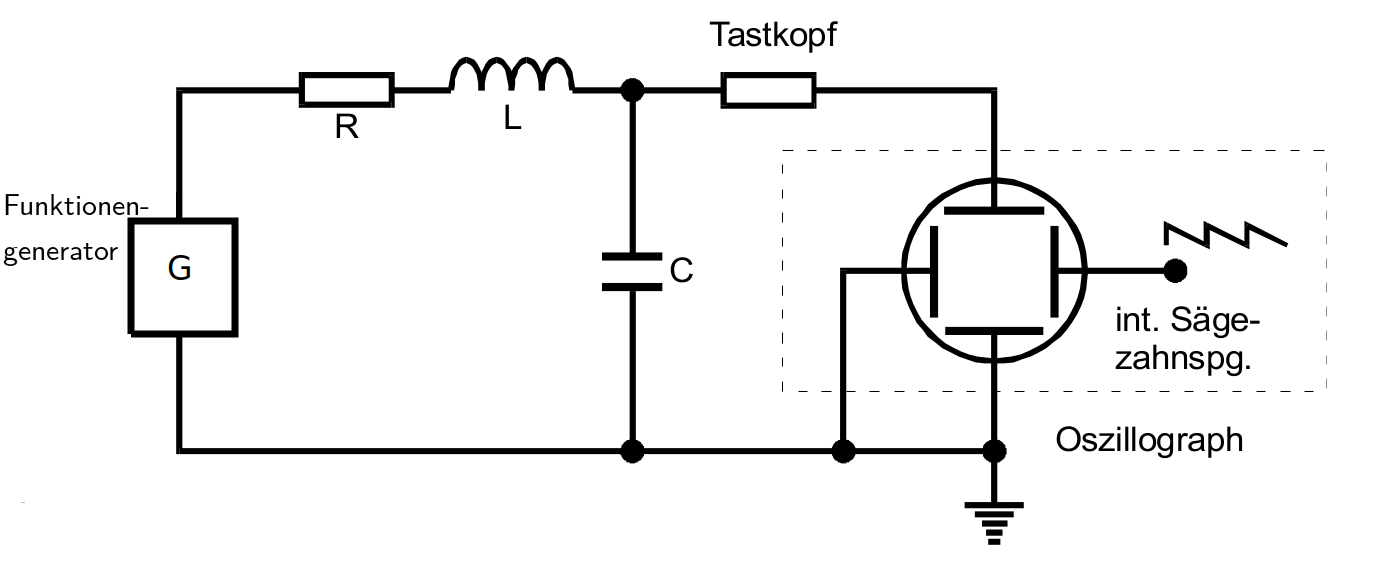
\includegraphics[width=0.9\textwidth]{Bilder/aufbaau.png}
	\caption{Prinzipieller Aufbau des RLC-Schwingkreises zur Untersuchung der zeitabhängigen Spannungsamplitude am Kondensator und des Widerstandes im aperiodischen Grenzfall. (vgl. \cite{Anleitung})}
	\label{fig:aufbau}
\end{figure}
Die Schaltung wird zunächst wie in Abbildung \eqref{fig:aufbau} aufgebaut. Diese besteht aus einem Funktionengenerator, dem RLC-Glied und dem Zweikanal-Oszilloskop mit dem Tastkopf zum Abgreifen der Kondensatorspannung.\\
Der Widerstand R kann im vorliegenden Schaltkreis zwischen drei verschiedenen Widerständen variiert werden. Die Widerstände $R_\text{1}$ und $R_\text{2}$ fest und der Widerstand $R_\text{3}$ ist als variierbarer Widerstand im Bereich von $0-10000\,\si{\ohm}$ realisiert.\\
An dem Funktionengenerator lassen sich verschiedene Spannungstypen realisieren. Unter anderem kann dieser die verwendete Nadelimpuls- sowie Sinusspannung erzeugen.\\
Die Größen der Induktivität $L$ und des Kondensators $C$ sind hierbei ebenso bekannt wie die Widerstände $R_\text{1}$ und $R_\text{2}$.

\begin{figure}
	\centering
	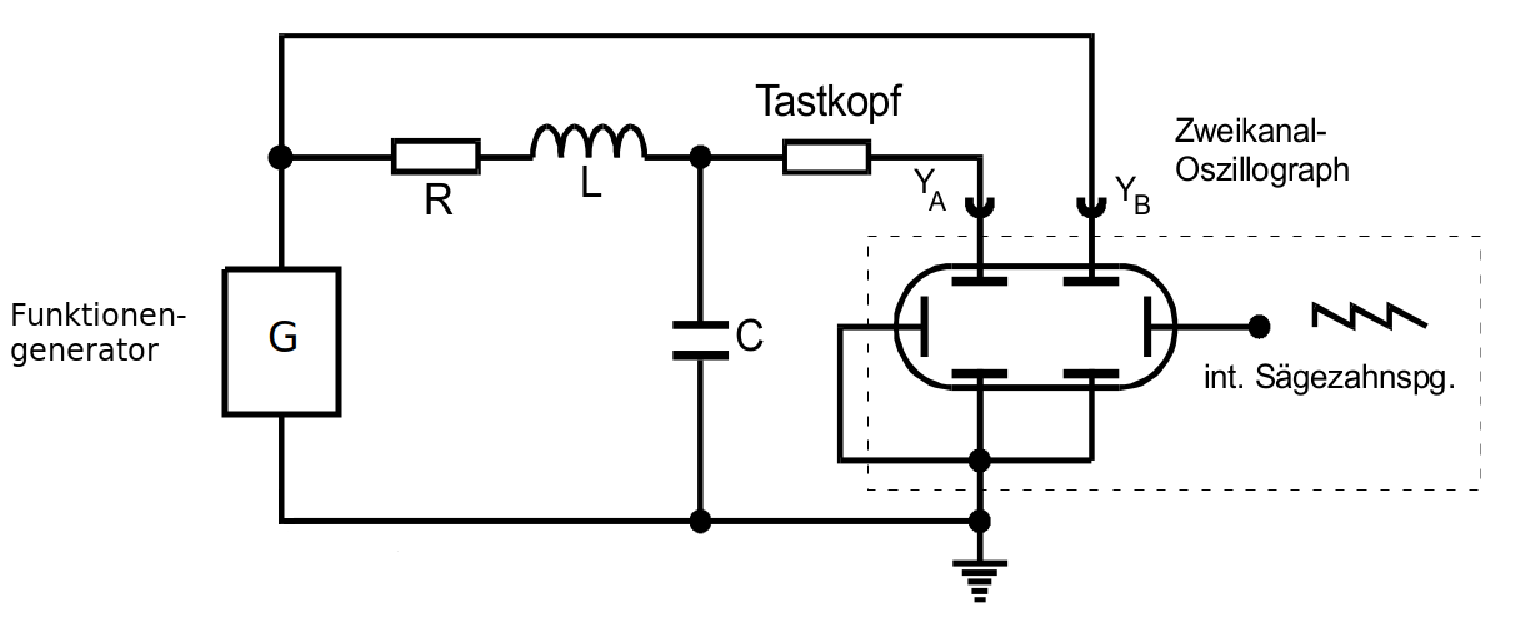
\includegraphics[width=0.9\textwidth]{Bilder/aufbauu.png}
	\caption{Aufbau des RLC-Schwingkreises zur Untersuchung der Frequenzabhängigkeit der Spannungsamplitude und der Phasenverschiebung zwischen Kondensatorspannung und Erregerspannung. (vgl. \cite{Anleitung})}
	\label{fig:aufbau2}
\end{figure}

Zur Messung der Frequenzabhängigkeit der Spannungsamplitude und der Phasenverschiebung zwischen Generatorspannung und Kondensatorspannung wird der Aufbau etwas modifiziert.\\
Das Zweikanal-Oszilloskop dient nun nicht mehr nur zum Aufzeichnen der Kondensatorspannung sondern der Versuchsaufbau wird wie in Abbildung \eqref{fig:aufbau2} dargestellt, verändert, sodass auf dem zweiten Kanal des Oszilloskops die Generatorspannung aufgenommen wird.
Die Generatorspannung und die Kondensatorspannung können nun zugleich am Oszilloskop aufgezeichnet werden.
